% main.tex: Keeping Syllables Whole Is Not Enough
% Compile with XeLaTeX (fastest; LuaLaTeX also works).
% On Overleaf: Menu > Compiler > XeLaTeX. Put acl.sty and acl_natbib.bst from the ACL template
% next to this file, and upload the figure PDFs into a folder called figures/.
\documentclass[11pt]{article}

% "review" for anonymous submission, "final" for camera-ready, "preprint" for arXiv.
\usepackage[final]{acl}

\usepackage{microtype}
\usepackage{graphicx}
\usepackage{booktabs}
\usepackage{adjustbox}
\usepackage{float}
\usepackage{amsmath}
\usepackage{xcolor}

% Fonts (XeLaTeX or LuaLaTeX). Plain fontspec is lighter and compiles faster than babel.
\usepackage{fontspec}
\setmainfont{TeX Gyre Termes}                                   % Times-like, as in the ACL template
\newfontfamily\devfont{Lohit Devanagari}[Script=Devanagari]      % Devanagari for Nepali examples
\newcommand{\np}[1]{{\devfont #1}}                               % Nepali text in Devanagari

\newcommand{\ap}{AksharaPiece}

\title{Keeping Syllables Whole Is Not Enough: Akshara-Aware Tokenization,\\
Corpus Typos, and Script-Aware Decoding for Nepali Language Models}

% Authors from different institutions: one column each, separated by \And.
\author{Sabin Bhattarai \\
  Pashchimanchal Campus \\
  Institute of Engineering \\
  Tribhuvan University, Pokhara, Nepal \\
  \texttt{pas078bct029@wrc.edu.np} \\\And
  Nabin Aadhikari \\
  Birendra Multiple Campus \\
  Institute of Science and Technology \\
  Tribhuvan University, Chitwan, Nepal \\
  \texttt{nabin2.805421@bimc.tu.edu.np} \\}

\begin{document}
\maketitle

% =====================================================================
\begin{abstract}
Subword tokenizers routinely cut Devanagari syllables (\emph{aksharas}) in half, separating a vowel sign or a halant from the consonant it belongs to. It seems natural to expect that a tokenizer which never does this would yield better Nepali language models. We test that expectation directly. We introduce \ap{}, a BPE tokenizer that treats each akshara as an unbreakable unit, and compare it with plain BPE under tightly matched conditions: the same 600\,MB of IndicCorp text, the same vocabulary size, and two architectures of equal size (a Llama-style Transformer and Mamba-2), each trained with three seeds. An audit of 12 tokenizers shows how widespread the problem is, with GPT-4's tokenizer cutting 99.5\% of Nepali words inside a syllable. Yet keeping syllables whole changes almost nothing downstream. Bits per byte differ by less than 0.4\% with no consistent direction, and news classification accuracy is identical. Generated text from every model contains fewer broken syllables than human-written text, and \ap{} does not reduce them further; with the Transformer it produces more. Analysing the errors explains why. Plain BPE models reproduce the typos already present in the training corpus, which we trace to legacy-font conversion, while \ap{} adds errors of its own through the way it encodes rare syllables. A simple script-aware decoding rule removes every broken syllable for both tokenizers without increasing non-words. We release the tokenizers, models, and evaluation code.\footnote{\raggedright Code: \url{https://github.com/USERNAME/aksharapiece}\newline Tokenizers and models: \url{https://huggingface.co/USERNAME}}
% PLACEHOLDER (links above): replace USERNAME once the GitHub and Hugging Face repositories are public. For anonymous review, use an anonymised link such as https://anonymous.4open.science
% or replace the footnote text with: Code and models will be released upon publication.
\end{abstract}

% =====================================================================
\section{Introduction}

Nepali is written in Devanagari, an abugida in which the unit a reader perceives is the \emph{akshara}: a consonant or consonant cluster together with its vowel sign and nasal marks. The word \np{नमस्ते} has three aksharas (\np{न}, \np{म}, \np{स्ते}) but six Unicode code points and eighteen UTF-8 bytes. Tokenizers built for English pay no attention to this structure. They regularly separate a vowel sign from its consonant or split a conjunct across two tokens, which also makes Nepali text several times more expensive to process than English \citep{petrov2023tokenizers,ahia-etal-2023-languages}.

It is tempting to conclude that the fix is a tokenizer that respects aksharas, and that such a tokenizer should give better models. Before building on that idea, we wanted to know whether it holds up when everything else is kept equal. This paper asks a simple question: \emph{if a tokenizer never splits an akshara, do Nepali language models get better?}

To answer it we built \ap{}, which maps every frequent akshara to a single symbol before running standard BPE, so that no merge can ever cross a syllable boundary. We then trained matched Transformer and Mamba-2 models on identical bytes with \ap{} and with plain BPE, and compared them on language modelling, on downstream classification, and on the well-formedness of the text they generate.

The answer turned out to be mostly no, and the reasons are more interesting than the headline. Our contributions are:

\begin{itemize}
  \item An audit of 12 tokenizers on Nepali, measuring token cost and how often each one cuts through a syllable (Section~\ref{sec:audit}).
  \item A controlled comparison of akshara-aware and plain BPE across two architectures and three seeds, which finds no reliable difference in bits per byte or classification accuracy (Sections~\ref{sec:lm} and~\ref{sec:cls}).
  \item A measurement of broken syllables in generated text, showing that well-trained models rarely produce them, and that a short script-aware decoding rule removes them entirely for any tokenizer (Section~\ref{sec:gen}).
  \item An error analysis linking the remaining broken syllables to legacy-font typos in IndicCorp and, for \ap{}, to its fallback for rare syllables (Section~\ref{sec:errors}).
\end{itemize}

% =====================================================================
\section{Related Work}

\paragraph{Tokenization across languages.}
Most current models rely on BPE \citep{sennrich-etal-2016-neural} or the unigram model in SentencePiece \citep{kudo-2018-subword,kudo-richardson-2018-sentencepiece}. Tokenizers trained mainly on English segment other languages poorly, which raises cost and can lower quality \citep{rust-etal-2021-good,petrov2023tokenizers,ahia-etal-2023-languages}. Whether tokenizer choice affects model quality has been examined from several directions. Some studies report clear effects \citep{bostrom-durrett-2020-byte,toraman2023impact}, while others find that compression and downstream quality are only loosely connected \citep{zouhar-etal-2023-tokenization,schmidt-etal-2024-tokenization,ali-etal-2024-tokenizer}. Byte-level models avoid the question altogether at the price of much longer sequences \citep{xue-etal-2022-byt5}.

\paragraph{Script-aware tokenization.}
Several recent proposals segment text along linguistic or orthographic units. Grapheme Pair Encoding builds merges on top of grapheme clusters for Tamil, Sinhala, and Hindi \citep{velayuthan-sarveswaran-2025-egalitarian}, and MYTE re-encodes bytes around morphemes to make costs fairer across languages \citep{limisiewicz-etal-2024-myte}. \ap{} follows the same intuition but uses aksharas, which match Devanagari orthography more closely than Unicode grapheme clusters do \citep{unicode15}. Our contribution is less the tokenizer itself than a careful test of whether this kind of tokenizer pays off.

\paragraph{Nepali language models.}
Nepali has encoder models such as NepBERTa \citep{timilsina-etal-2022-nepberta} and the models compared by \citet{maskey-etal-2022-nepali}, and it is covered by multilingual Indic models such as MuRIL \citep{khanuja2021muril} and IndicBERT~v2, whose pretraining corpus IndicCorp~v2 we also use \citep{doddapaneni-etal-2023-towards}. Closest to our work, \citet{luitel-etal-2025-perplexity} compare tokenization schemes for small Nepali sequential models and find that lower perplexity does not predict better fine-tuning. Our results agree with theirs and extend the comparison to state-space models and to generated text.

\paragraph{Constrained decoding.}
Restricting which tokens a model may emit is a standard way to enforce structure at inference time, for example with grammars or regular expressions \citep{geng-etal-2023-grammar,willard2023efficient}. Our script-aware rule is a very small instance of this idea, aimed at Devanagari orthography.

% =====================================================================
\section{Method}

\subsection{Aksharas}
We split text into aksharas with a single regular expression over Unicode code points. An akshara is either (i) zero or more half consonants (consonant, optional nukta, halant, optional ZWJ), followed by a base consonant, an optional nukta, and then either a visible halant or any vowel signs, and finally any nasal or visarga marks; or (ii) an independent vowel with optional marks. Every other character, including Latin letters, digits, and punctuation, forms its own unit, and a sign with nothing to attach to becomes a unit of its own. This keeps \np{क्षे}, \np{स्त्री}, and word-final \np{छन्} intact, and lets us detect two kinds of malformed syllables: a dependent sign with no base (for example after a space or a halant), and more than one vowel sign on the same syllable.

Before tokenization, all text is normalised to NFC. Invisible characters such as the soft hyphen and byte order mark are removed, and three vowel-sign sequences that commonly result from font conversion (\np{ा}+\np{े}, \np{ा}+\np{ै}, \np{े}+\np{ा}) are repaired.

\subsection{\ap{}}
\ap{} wraps a standard BPE tokenizer. Before training, we count aksharas in the tokenizer training text and keep the most frequent ones until they cover 99.9\% of all occurrences, which gives 2,963 aksharas for our 16k vocabulary. Each kept akshara is mapped to a single private-use code point, so BPE sees it as one indivisible character and can only merge whole aksharas into larger tokens. Rarer aksharas are split into their consonant cluster and their vowel signs, each of which can still be learned as a symbol. Decoding reverses the mapping, so \ap{} is lossless.

On the training text, \ap{} needs 1.6\% more tokens than plain BPE with the same vocabulary size (12.31 versus 12.50 bytes per token), because some vocabulary slots go to single aksharas instead of longer merges.

\subsection{Script-aware decoding}
\label{sec:constrained}
As a decoding-time alternative, we block tokens that would create a malformed syllable. Each character belongs to one of seven classes (consonant, nukta, vowel sign, nasal mark, halant, independent vowel, other). A token whose first character is a dependent sign is allowed only after a compatible character: a vowel sign or halant only after a consonant or nukta, a nukta only after a consonant, and a nasal mark only after a consonant, nukta, vowel sign, or independent vowel. Tokens that are malformed on their own, such as a token holding two vowel signs, are never allowed. The rule needs only the class of the last generated character and a precomputed boolean mask over the vocabulary, so it costs almost nothing at inference time and works with any tokenizer.

% =====================================================================
\section{Experimental Setup}

\subsection{Data}
We use the Nepali portion of IndicCorp~v2 \citep{doddapaneni-etal-2023-towards}. From the first 1.5\,GB of the file we remove URLs, HTML, and private-use characters, drop empty and very short lines and lines in which fewer than 60\% of letters are Devanagari, remove exact duplicates and any sentence that also appears in FLORES, and shuffle. This leaves 2.5 million lines, which we split into 20\,MB of held-out text, 100\,MB for training tokenizers, and the remainder for language-model pretraining. Every language model sees the same first 600\,MB of pretraining text, and bits per byte is measured on the same 5\,MB of held-out text.

\subsection{Tokenizers}
For the main experiments we train plain BPE and \ap{} BPE with a 16k vocabulary on the same 100\,MB, using the same trainer and the same Metaspace pre-tokenization. For the audit we add 32k versions and ten existing tokenizers: GPT-4 and GPT-4o \citep{tiktoken}, Llama~3.2 \citep{grattafiori2024llama3}, Qwen~2.5 \citep{qwen25}, Mistral Tekken, Gemma~3 \citep{gemma3}, Sarvam-1 \citep{sarvam1}, MuRIL \citep{khanuja2021muril}, IndicBERT~v2 \citep{doddapaneni-etal-2023-towards}, and a Nepali SentencePiece model \citep{nepalitokenizers}. The audit uses the 6,511 distinct Nepali sentences in the FLORES Nepali--English sets \citep{guzman-etal-2019-flores}.

\subsection{Models and training}
Both architectures use a model width of 512, tied input and output embeddings, and about 27M non-embedding parameters. The Transformer \citep{vaswani2017attention} follows the Llama recipe, with 8 layers, 8 heads, rotary positions \citep{su2024roformer}, RMSNorm \citep{zhang2019rmsnorm}, and SwiGLU feed-forward blocks \citep{shazeer2020glu} (27.3M parameters). The Mamba-2 model \citep{gu2023mamba,dao2024transformers} has 16 layers with state size 64, head dimension 64, and expansion 2 (26.5M parameters); we implement its chunked scan in plain PyTorch and run it in float32. All models train for one pass over the 600\,MB (about 48M tokens) with sequences of 1,024 tokens, 16 sequences per step, AdamW \citep{loshchilov2019adamw} with peak learning rate $10^{-3}$, 3\% warmup, and cosine decay. We train three seeds per configuration on free Kaggle T4 GPUs. Seed 0 used bfloat16, and seeds 1 and 2 used float16, which is native on the T4. A Transformer run takes about 30 minutes and a Mamba-2 run about 95 minutes. Appendix~\ref{app:hparams} lists all settings.


\subsection{Evaluation}
\paragraph{Bits per byte.} Because the tokenizers split text differently, we report the total negative log-likelihood of the held-out text divided by its size in UTF-8 bytes \citep{gao2020pile}. To compare tokenizers within a seed, we use a paired bootstrap over held-out lines \citep{koehn-2004-statistical}.

\paragraph{Classification.} We fine-tune every pretrained model on np20ng \citep{np20ng}, a Nepali news dataset with 20 topics, using 1,000 training and 200 test articles per topic. Each article is cut to its first 600 characters, so that every tokenizer sees exactly the same text. A linear layer on mean-pooled final hidden states is trained together with the whole model for three epochs.

\paragraph{Generated text.} Each model continues 3,000 sentence openings, made of the first six words of distinct FLORES sentences, for up to 64 tokens with nucleus sampling \citep{holtzman2020curious} ($p=0.95$, temperature 0.8). We count malformed syllables in the generated part and report them per 1,000 syllables. We also report the share of generated words that occur fewer than three times in 200\,MB of IndicCorp drawn from far beyond the training portion. Human-written text from another distant part of the corpus is scored the same way as a reference.

One detail matters a great deal here. A continuation must be scored together with its opening, because a model may legitimately extend the last word of the opening: \np{बसाइ} followed by \np{ँसराइ} gives the correct word \np{बसाइँसराइ}. In a pilot run, scoring continuations on their own counted half of plain BPE's ``broken'' syllables in exactly this way, which made plain BPE look twice as bad as it was.

% =====================================================================
\section{Results}

\subsection{How tokenizers treat Nepali}
\label{sec:audit}

\begin{figure*}[t]
  \centering
  % PLACEHOLDER: upload figures/fig1_tokenizer_audit.pdf
  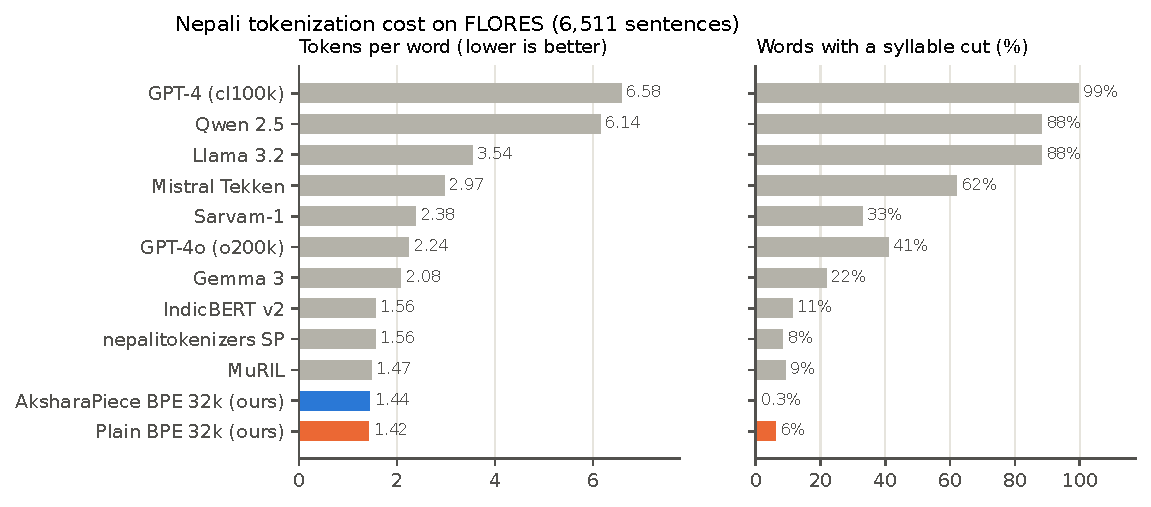
\includegraphics[width=\textwidth]{figures/fig1_tokenizer_audit.pdf}
  \caption{Tokens per Nepali word (left) and share of words with at least one token boundary inside an akshara (right), on 6,511 FLORES sentences. Our two 32k tokenizers are shown in colour.}
  \label{fig:audit}
\end{figure*}

Figure~\ref{fig:audit} shows that general-purpose tokenizers handle Nepali very differently. GPT-4's tokenizer needs 6.58 tokens per word and cuts through a syllable in 99.5\% of words, which makes Nepali 4.6 times as expensive as the English side of the same sentences. GPT-4o and Gemma~3 do much better, at about two tokens per word, but they still break 41\% and 22\% of words. Sarvam-1, a model for Indian languages, breaks a third of Nepali words. Its model card does not list Nepali among its languages. Tokenizers trained on Indic or Nepali text (MuRIL, IndicBERT~v2, and the Nepali SentencePiece model) reach about 1.5 tokens per word but still break 8 to 11\% of words. Our plain BPE, trained only on Nepali, is the most compact at 1.42 tokens per word and breaks 6.2\% of words. \ap{} reduces that to 0.3\% while needing only 1.5\% more tokens.

So syllable-breaking is common, and it can be almost eliminated at little cost. The rest of the paper asks whether doing so helps.

\subsection{Language modelling}
\label{sec:lm}

\begin{table}[t]
  \centering
  \small
  \begin{adjustbox}{max width=\columnwidth}
  \begin{tabular}{lccc}
    \toprule
    & Plain BPE & \ap{} & Difference \\
    \midrule
    Transformer & 0.5152 {\scriptsize $\pm$0.0017} & 0.5136 {\scriptsize $\pm$0.0029} & $-0.31\%$ {\scriptsize $\pm$0.46} \\
    Mamba-2     & 0.5070 {\scriptsize $\pm$0.0004} & 0.5065 {\scriptsize $\pm$0.0004} & $-0.09\%$ {\scriptsize $\pm$0.08} \\
    \bottomrule
  \end{tabular}
  \end{adjustbox}
  \caption{Bits per byte on held-out IndicCorp text (lower is better), mean $\pm$ standard deviation over three seeds.}
  \label{tab:bpb}
\end{table}

\begin{figure*}[t]
  \centering
  % PLACEHOLDER: upload figures/fig2_bpb_difference.pdf
  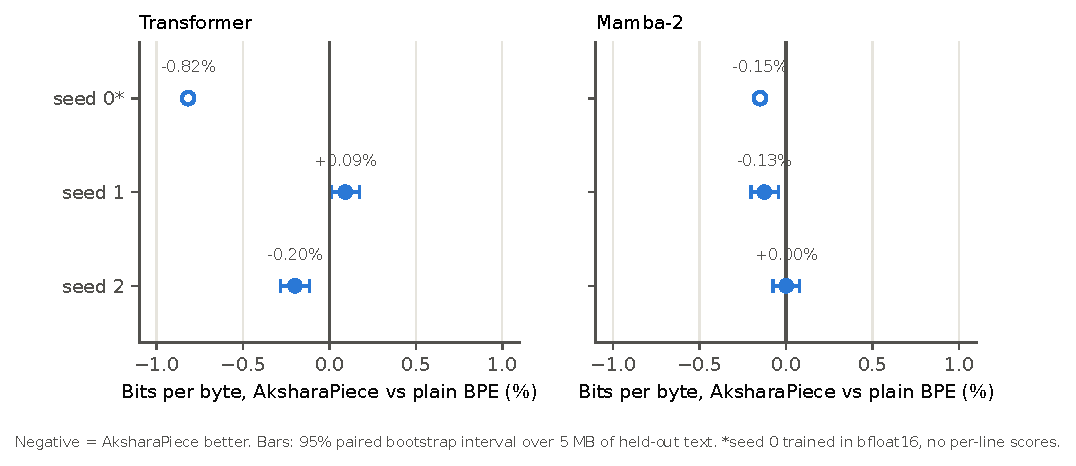
\includegraphics[width=0.95\textwidth]{figures/fig2_bpb_difference.pdf}
  \caption{Relative difference in bits per byte for each seed. Error bars are 95\% paired bootstrap intervals over held-out lines (not available for seed 0).}
  \label{fig:bpb}
\end{figure*}

Table~\ref{tab:bpb} gives the averages and Figure~\ref{fig:bpb} the individual seeds. \ap{} is slightly ahead on average, but the gap is smaller than the variation between seeds. For the Transformer, one seed favours \ap{} by 0.82\%, another by 0.20\%, and the third favours plain BPE by 0.09\%. The bootstrap intervals show that each of these per-seed differences is real for that particular run, yet the direction changes from run to run. For Mamba-2, the differences stay within 0.15\%. Taken together, we find no reliable effect of keeping aksharas whole on how well the models predict Nepali text, and no sign of harm either.

Across architectures, Mamba-2 reaches lower bits per byte than the Transformer with the same parameter budget (0.507 against 0.514), although in our plain PyTorch implementation it trains about three times more slowly.

\subsection{Downstream classification}
\label{sec:cls}

\begin{table}[t]
  \centering
  \small
  \begin{adjustbox}{max width=\columnwidth}
  \begin{tabular}{lcc}
    \toprule
    & Plain BPE & \ap{} \\
    \midrule
    Transformer & 83.43 {\scriptsize $\pm$0.11} & 83.56 {\scriptsize $\pm$0.37} \\
    Mamba-2     & 84.06 {\scriptsize $\pm$0.51} & 84.14 {\scriptsize $\pm$0.48} \\
    \bottomrule
  \end{tabular}
  \end{adjustbox}
  \caption{Test accuracy (\%) on 20-class np20ng news classification, mean $\pm$ standard deviation over two pretraining seeds. Macro-F1 follows accuracy within 0.1 points.}
  \label{tab:cls}
\end{table}

Fine-tuning tells the same story (Table~\ref{tab:cls}; per-seed results in Appendix~\ref{app:cls}). The two tokenizers are within 0.15 points of each other for both architectures, and within each architecture the spread between pretraining seeds is larger than the gap between the tokenizers. This matches the observation of \citet{luitel-etal-2025-perplexity} that differences visible during pretraining often disappear after fine-tuning.



\subsection{Broken syllables in generated text}
\label{sec:gen}

\begin{figure*}[t]
  \centering
  % PLACEHOLDER: upload figures/fig4_generation_validity.pdf
  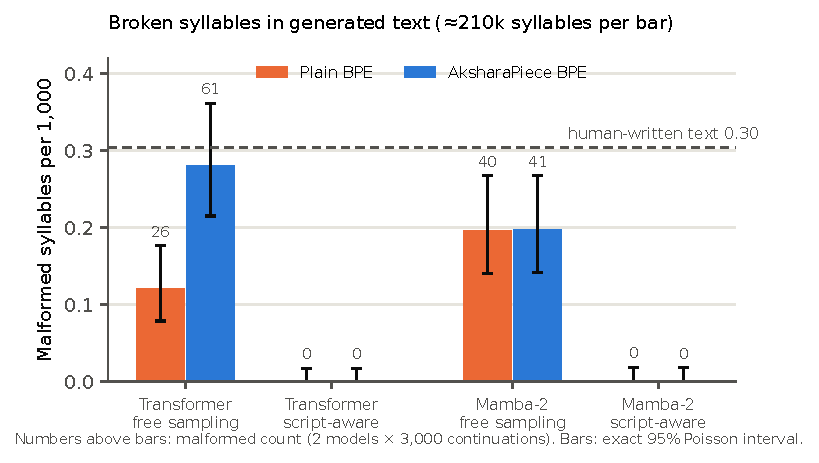
\includegraphics[width=0.78\textwidth]{figures/fig4_generation_validity.pdf}
  \caption{Malformed syllables per 1,000 generated syllables, pooled over two seeds and 3,000 continuations per model. Error bars are exact 95\% Poisson intervals; numbers give the raw counts. The dashed line is human-written text.}
  \label{fig:gen}
\end{figure*}

\begin{table}[t]
  \centering
  \small
  \begin{adjustbox}{max width=\columnwidth}
  \begin{tabular}{llcc}
    \toprule
    & Decoding & Plain BPE & \ap{} \\
    \midrule
    Transformer & free        & 26 & 61 \\
                & script-aware & 0  & 0  \\
    Mamba-2     & free        & 40 & 41 \\
                & script-aware & 0  & 0  \\
    \midrule
    \multicolumn{2}{l}{Non-words, free}         & 4.09\% & 4.23\% \\
    \multicolumn{2}{l}{Non-words, script-aware} & 4.04\% & 4.14\% \\
    \bottomrule
  \end{tabular}
  \end{adjustbox}
  \caption{Malformed syllables in about 210,000 generated syllables per cell, and the share of generated words not found in a 200\,MB reference corpus. Human-written text has 0.30 malformed syllables per 1,000 and 4.24\% non-words.}
  \label{tab:gen}
\end{table}

If keeping syllables whole helps anywhere, it should help with the text a model writes, since a model that only ever emits whole aksharas has fewer ways to produce an invalid one. Figure~\ref{fig:gen} and Table~\ref{tab:gen} show that this is not what happens.

First, broken syllables are rare for every model. All eight models produce between 0.12 and 0.28 malformed syllables per 1,000, fewer than the 0.30 found in human-written IndicCorp text. Second, \ap{} does not reduce them. With Mamba-2 the two tokenizers are tied (40 against 41), and with the Transformer \ap{} produces more than twice as many (61 against 26; exact rate test $p=0.0002$). Pooled over both architectures, \ap{} is slightly worse ($p=0.009$). Third, script-aware decoding brings the count to zero for every model, and the share of non-words stays at the level of human text.

We should add a caution about sample size. In an earlier run with 300 openings per model, \ap{} appeared to produce five times fewer broken syllables. That result came from very small counts (5 against 24) and from the scoring problem described above, and it disappeared once we generated ten times more text and scored it correctly. In a sanity check with tiny, heavily undertrained models (Appendix~\ref{app:tiny}), \ap{} did reduce broken syllables substantially, which suggests its advantage may matter mainly when models have seen little data.

\subsection{Where broken syllables come from}
\label{sec:errors}

\begin{table}[t]
  \centering
  \small
  \begin{adjustbox}{max width=\columnwidth}
  \begin{tabular}{lccc}
    \toprule
    Error type & Corpus & Plain & \ap{} \\
    \midrule
    Same vowel sign twice     & 25 & 27 & 18 \\
    Two different vowel signs & 26 & 18 & 18 \\
    Nasal before vowel sign   & 13 & 14 & 2  \\
    Sign after halant         & 6  & 8  & 21 \\
    Sign at word start        & 10 & 12 & 24 \\
    Other                     & 20 & 21 & 19 \\
    \midrule
    Count                     & 5,572 & 66 & 102 \\
    \bottomrule
  \end{tabular}
  \end{adjustbox}
  \caption{Share (\%) of each kind of malformed syllable in 100\,MB of IndicCorp training text and in text generated with free sampling.}
  \label{tab:errors}
\end{table}

\begin{figure*}[t]
  \centering
  % PLACEHOLDER: upload figures/fig6_error_types.pdf
  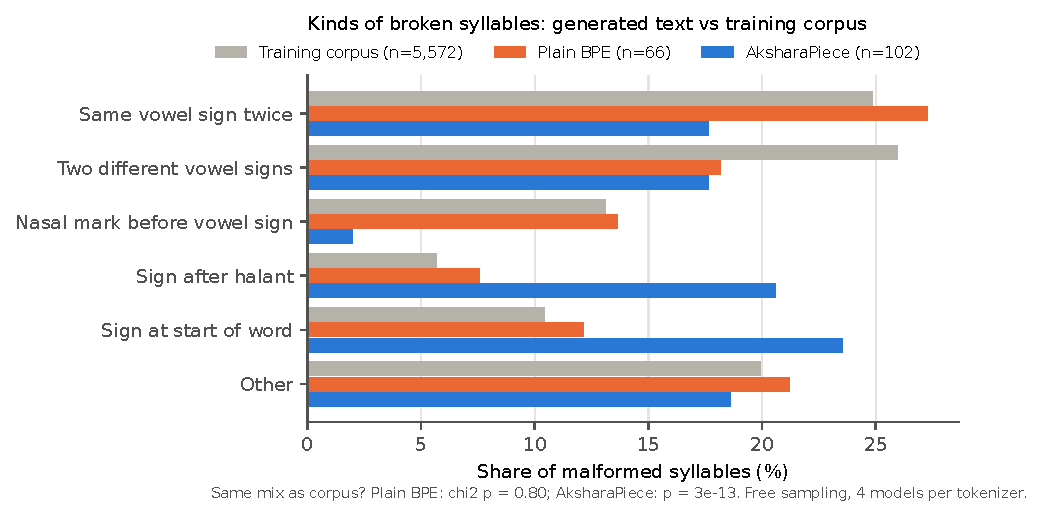
\includegraphics[width=0.8\textwidth]{figures/fig6_error_types.pdf}
  \caption{Kinds of malformed syllables in the training corpus and in generated text. Plain BPE models reproduce the corpus mix; \ap{} models do not.}
  \label{fig:errors}
\end{figure*}

To understand these errors we classified every malformed syllable in 100\,MB of the training text and in all generated text (Table~\ref{tab:errors}, Figure~\ref{fig:errors}).

\paragraph{The corpus contains them.} IndicCorp Nepali has 0.32 malformed syllables per 1,000, and 2.7\% of its lines contain at least one. Most look like leftovers from converting text typed in legacy fonts such as Preeti into Unicode: a vowel sign typed twice (\np{दुुई}), a nasal mark typed before the vowel sign (\np{हँुदै} for \np{हुँदै}), extra vowel signs (\np{भएकोे}), or the \np{र} of a conjunct placed in the wrong order (\np{दु्रत} for \np{द्रुत}). About 7.5\% of the flagged cases are clock times such as \np{५ः३०}, where the visarga stands in for a colon; this is a writing convention rather than an error. Two conservative repair rules, removing a repeated vowel sign and moving a nasal mark after the vowel sign, fix about a third of the cases (Appendix~\ref{app:typos}).



\paragraph{Plain BPE copies them.} The mix of error types produced by plain BPE models cannot be told apart from the corpus mix ($\chi^2$ test, $p=0.80$). Its errors are the corpus typos themselves, such as \np{बंैक} and \np{गर्नुुपर्छ}. The tokenizer is not inventing these errors; the model learns them from the data.

\paragraph{\ap{} makes different ones.} \ap{} models almost never reproduce the nasal-order typo (2\% of their errors), which needs a split inside an akshara that \ap{} cannot represent. Instead, their errors are dominated by a vowel sign placed after a halant (\np{झ्ेख}, \np{सञ्ार}) or at the start of a word, and their mix differs clearly from the corpus ($p<10^{-12}$). These errors come from \ap{}'s own vocabulary. To handle rare aksharas, it contains bare vowel signs as tokens, and it contains half-consonant symbols ending in a halant. Nothing stops a model from placing one after the other. Because bare vowel signs appear only in rare contexts during training, the model sees them seldom and, we suspect, learns their use poorly.

% =====================================================================
\section{Discussion}

Our results point to a gap between a tokenizer's properties and a model's behaviour. A guarantee that the tokenizer never splits an akshara is a statement about segmentation. It does not prevent a model from producing an invalid akshara, because invalid sequences can still be built from valid pieces, and because the training data contains invalid text that the model learns to imitate. In our setting the model learns where syllables begin and end about equally well whether or not the tokenizer marks them. This is consistent with findings that compression and segmentation quality are weak predictors of model quality \citep{schmidt-etal-2024-tokenization,ali-etal-2024-tokenizer}.

For practitioners building Nepali or other Devanagari models, three lessons follow. First, cleaning the training data is likely to matter more than the choice between these tokenizers: the broken syllables that remain in model output largely reflect typos in the corpus. Second, if an akshara-aware tokenizer is used, rare syllables need a fallback that cannot expose bare vowel signs. Third, when well-formed output is required, script-aware decoding is a cheap and complete fix that works with any tokenizer.

Akshara-aware tokenization still has things going for it. It costs only 1.5 to 1.6\% more tokens, never hurts language modelling or classification in our experiments, and produces segments that people can read and inspect. It also seemed to help the tiny, undertrained models in our sanity check. Whether its advantages grow in very low-data settings, or shrink further with scale, is an open question.

% =====================================================================
\section{Conclusion}

We tested whether a tokenizer that keeps Devanagari syllables whole leads to better Nepali language models. Under controlled conditions with two architectures and several seeds, it did not: bits per byte and classification accuracy were unchanged, and generated text was no cleaner. The broken syllables that models do produce come mostly from typos in the training corpus, plus, for \ap{}, from the way it encodes rare syllables, and a simple decoding rule removes all of them. We hope these results, together with the released tokenizers, models, and code, help others choose where effort on Nepali language technology is most likely to pay off.

% =====================================================================
\section*{Limitations}

Our models are small (about 35M parameters including embeddings) and are trained on 600\,MB of text, so the conclusions may not carry over to models that are orders of magnitude larger or trained much longer. We study a single language and a single corpus; other Devanagari languages, other scripts, and cleaner corpora could behave differently. We compare against plain BPE only and use one vocabulary size (16k) for the controlled experiments. The classification experiment uses one task and two seeds, and generation quality is measured with automatic, orthography-level checks rather than human judgement of fluency or meaning. Seed 0 was trained in bfloat16 and seeds 1 and 2 in float16, which adds a small source of variation. Finally, the Mamba-2 implementation is our own plain PyTorch version, which is slower than the official kernels, although it computes the same function.

\section*{Ethics Statement}

We use publicly released data: IndicCorp~v2 (CC0), FLORES, and np20ng, under their respective licences. The corpora are web-crawled and may contain offensive content or personal information; we did not filter for these beyond the cleaning described above, and our small models are released for research use only. All training and evaluation ran on free cloud GPUs, totalling about 25 GPU hours.

% =====================================================================
\bibliography{references}





\onecolumn   % one-column appendix: each table and figure stays with its own section
\appendix

\section{Hyperparameters}
\label{app:hparams}

Table~\ref{tab:hparams} lists the settings shared by all runs.

\begin{table}[H]
  \centering
  \small
  \begin{adjustbox}{max width=\columnwidth}
  \begin{tabular}{lcc}
    \toprule
    & Transformer & Mamba-2 \\
    \midrule
    Layers & 8 & 16 \\
    Model width & 512 & 512 \\
    Heads / head dim & 8 / 64 & 16 / 64 \\
    Feed-forward / expansion & SwiGLU, $3\times$ & $2\times$ \\
    State size & -- & 64 \\
    Non-embedding params & 27.3M & 26.5M \\
    Embedding params (tied) & 8.2M & 8.2M \\
    \midrule
    Vocabulary & \multicolumn{2}{c}{16,000 + 1 line separator} \\
    Sequence length & \multicolumn{2}{c}{1,024} \\
    Sequences per step & \multicolumn{2}{c}{16} \\
    Training text & \multicolumn{2}{c}{600\,MB, one pass} \\
    Optimiser & \multicolumn{2}{c}{AdamW, $\beta=(0.9, 0.95)$, wd 0.1} \\
    Learning rate & \multicolumn{2}{c}{$10^{-3}$, 3\% warmup, cosine to 10\%} \\
    Gradient clipping & \multicolumn{2}{c}{1.0} \\
    Precision & \multicolumn{2}{c}{bf16 (seed 0), fp16 (seeds 1--2)} \\
    \midrule
    Fine-tuning & \multicolumn{2}{c}{3 epochs, batch 32, AdamW, lr $10^{-4}$} \\
    Generation & \multicolumn{2}{c}{top-$p$ 0.95, temperature 0.8, 64 tokens} \\
    \bottomrule
  \end{tabular}
  \end{adjustbox}
  \caption{Model, training, fine-tuning, and generation settings.}
  \label{tab:hparams}
\end{table}

\section{Classification results by seed}\label{app:cls}

Figure~\ref{fig:cls} shows the np20ng test accuracy of every fine-tuned model. Within each architecture, the spread between pretraining seeds is larger than the gap between the two tokenizers.

\begin{figure}[H]
  \centering
  % PLACEHOLDER: upload figures/fig3_classification.pdf
  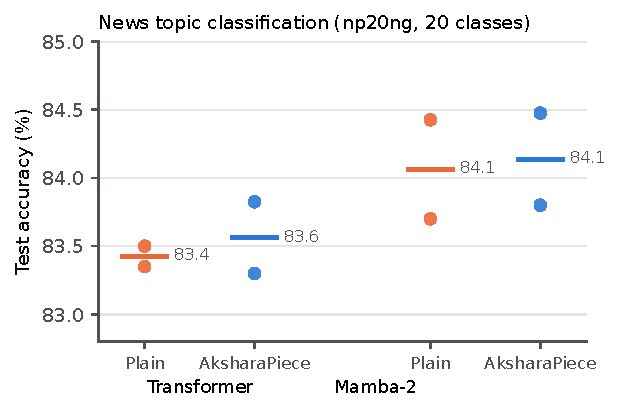
\includegraphics[width=0.6\textwidth]{figures/fig3_classification.pdf}
  \caption{np20ng test accuracy for each pretraining seed (dots) and their mean (bars).}
  \label{fig:cls}
\end{figure}

\section{Typos in the training corpus}\label{app:typos}

Figure~\ref{fig:typos} breaks down the malformed syllables we found in 100\,MB of training text by type. Two simple repair rules fix about a third of these cases. The first rule collapses a vowel sign that is repeated immediately after itself; the second swaps a candrabindu or anusvara with a vowel sign that directly follows it. The cases they leave behind are mostly other vowel-sign combinations such as \np{ोे}, a misplaced \np{र} inside a conjunct, and the clock times mentioned above.

\begin{figure}[H]
  \centering
  % PLACEHOLDER: upload figures/fig5_corpus_typos.pdf
  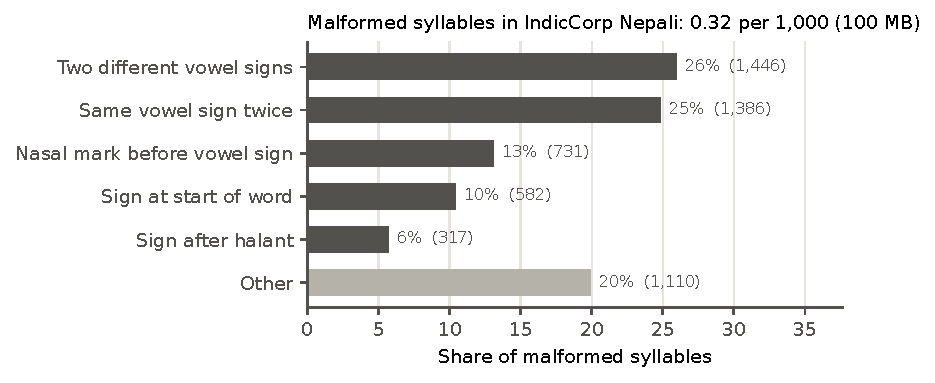
\includegraphics[width=0.68\textwidth]{figures/fig5_corpus_typos.pdf}
  \caption{Kinds of malformed syllables in 100\,MB of IndicCorp Nepali training text (5,572 cases in 17.5 million syllables).}
  \label{fig:typos}
\end{figure}

\section{Sanity check with tiny models}\label{app:tiny}

While developing the evaluation, we trained tiny models (width 64, two layers, 4k vocabulary) on a small amount of text on a CPU. With free sampling, plain BPE models produced 14 to 19 malformed syllables per 1,000, while \ap{} models produced 1 to 3.5, roughly a five-fold reduction. Script-aware decoding again removed all of them. These models are far too small to draw conclusions from, but the contrast with the full-size models suggests that the benefit of akshara-aware tokenization fades as models learn the orthography from data.

\end{document}
